% ======================================================
%  1 — MOTIVATION
% ======================================================
\section{Why AI? Why Crosswords?}

% --- 1.1 History timeline ---
\begin{frame}{Technology Has Never ``Revolutionized'' Education}
  \begin{center}
    \begin{tikzpicture}[
      yearnode/.style={circle, fill=unisired!15, minimum size=1cm, font=\small\bfseries, text=unisired},
      technode/.style={font=\small, text=darktext, align=center},
    ]
    \draw[line width=1pt, graytext] (0,0) -- (12,0);
    \node[yearnode] at (0.5, 0) {1922};
    \node[technode, above=0.35cm] at (0.5, 0) {Film};
    \node[yearnode] at (3, 0) {1930s};
    \node[technode, below=0.35cm] at (3, 0) {Radio};
    \node[yearnode] at (5.5, 0) {1950s};
    \node[technode, above=0.35cm] at (5.5, 0) {Television};
    \node[yearnode] at (8, 0) {1980s};
    \node[technode, below=0.35cm] at (8, 0) {Computers};
    \node[yearnode] at (10.5, 0) {2020s};
    \node[technode, above=0.35cm] at (10.5, 0) {AI / LLMs};
    \end{tikzpicture}
  \end{center}
  \vfill
  \only<1>{%
    \begin{quote}
      \small\color{graytext}%
      ``The motion picture is destined to revolutionize our educational system
      and [\ldots] supplant the use of textbooks.''\\
      \upshape\hfill --- \textbf{Thomas Edison}
    \end{quote}
  }%
  \only<2>{%
    \begin{quote}
      \small\color{graytext}%
      `` is going to make school so attractive that a big army with swords and guns couldn’t keep boys and girls out of it.''\\
      \upshape\hfill --- \textbf{Thomas Edison}
      \hfill{\scriptsize (on children's enthusiasm for film-based lessons)}
    \end{quote}
  }%
  \only<3>{%
    \begin{quote}
      \small\color{graytext}%
      ``In 50 years, there will be only 10 institutions in the world
      delivering higher education.''\\
      \upshape\hfill --- \textbf{Sebastian Thrun, 2012}
      \hfill{\scriptsize}
    \end{quote}
    \vspace{0.3em}
    \centering{\small\color{graytext}\textit{Spoiler: it did not.}}
  }%
\end{frame}

% --- 1.1b Jobs pivot ---
\begin{frame}{Even the Man Who Gave Computers to Schools Said\ldots}
  \begin{columns}[c]
    \column{0.35\textwidth}
      \centering
      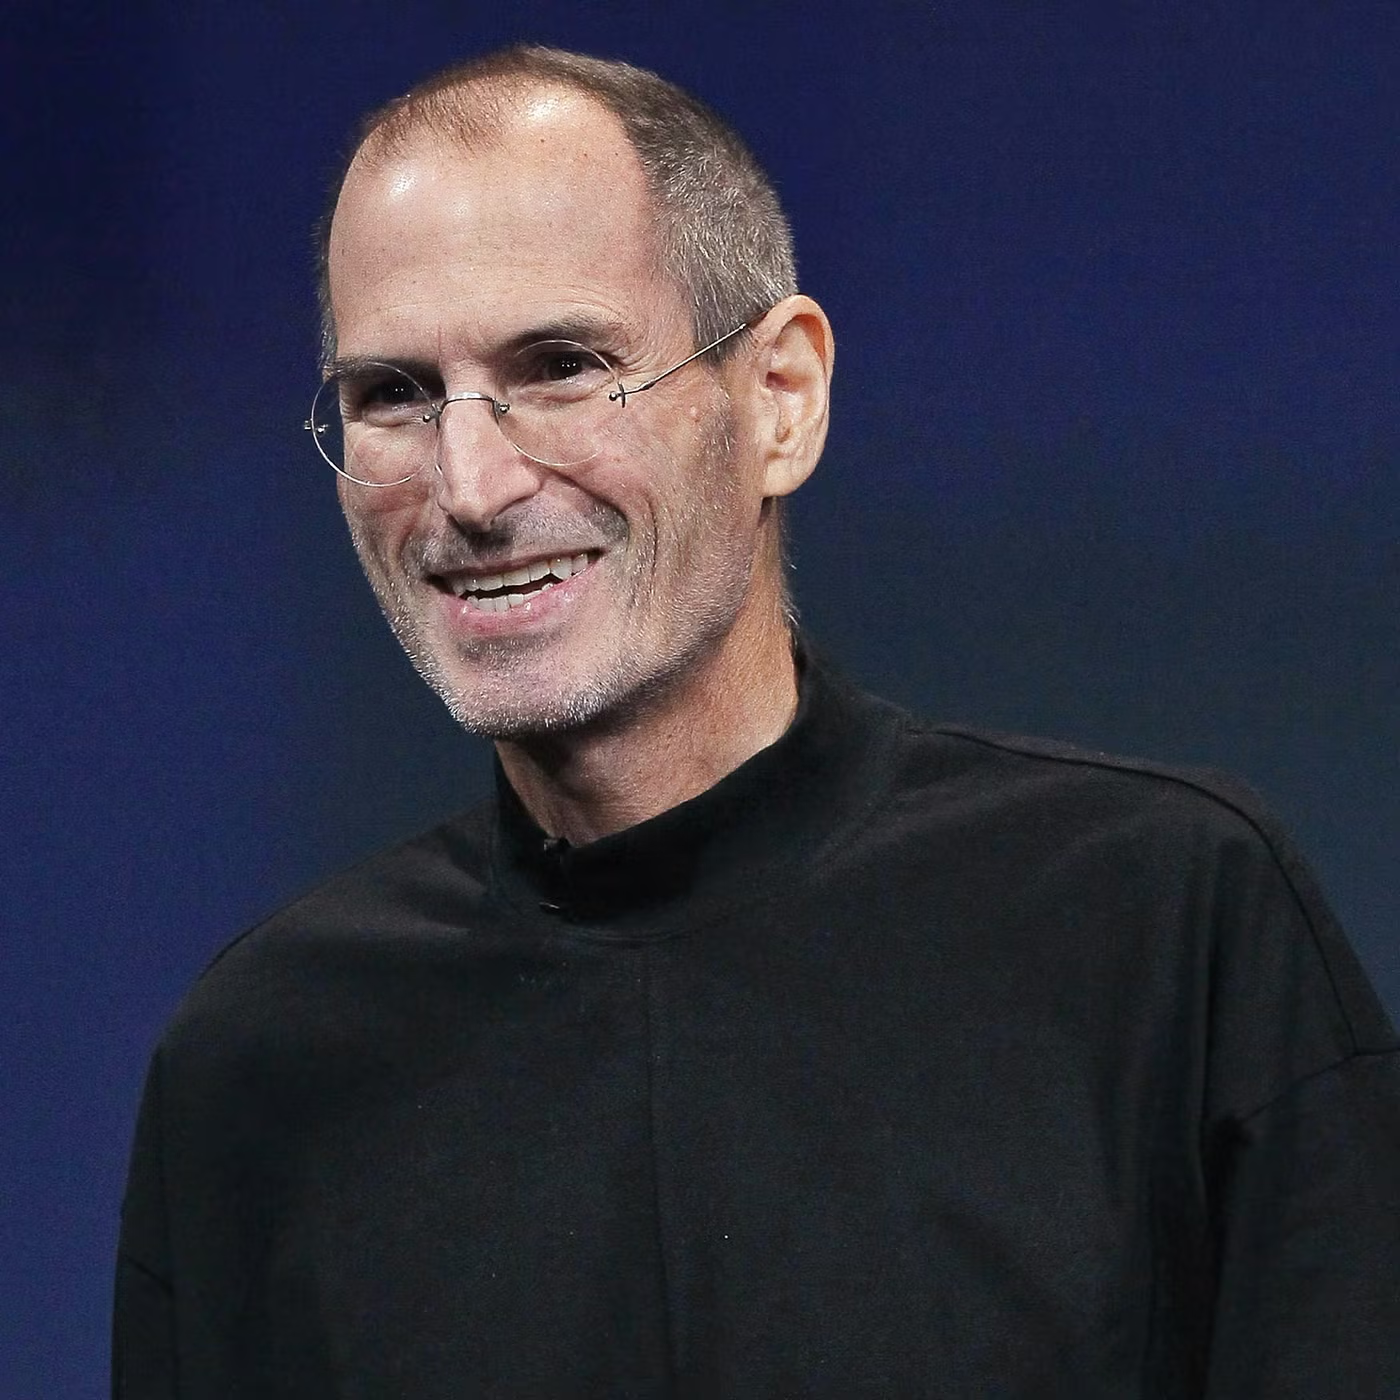
\includegraphics[width=0.82\textwidth]{figures/jobs.png}\\[0.3em]
      {\small\color{graytext} Steve Jobs, 1996}
    \column{0.65\textwidth}
      \vspace{0.5em}
      \begin{quote}
        \color{darktext}
        ``What's wrong with education cannot be fixed with technology.
        No amount of technology will make a dent.
        \textbf{The problems are sociopolitical.}''
      \end{quote}
      \vspace{1.2em}
      \only<2>{%
        \begin{quote}
          \color{darktext}
          ``The most important thing is a \textbf{person}.
          A person who incites your curiosity and feeds your curiosity;
          and machines cannot do that in the same way that people can.''
        \end{quote}
        \vspace{0.5em}
        \hfill{\scriptsize\color{graytext} --- Jobs, interview with Daniel Morrow, 1995}
      }%
  \end{columns}
\end{frame}

% --- 1.2 AI evidence ---
\begin{frame}{Yet AI \textit{Does} Improve Learning}
  \begin{columns}[c]
    \column{0.5\textwidth}
      \begin{center}
        {\fontsize{56}{66}\selectfont\color{unisired}\textbf{+0.87}}\\[0.3em]
        {\large standard deviations}\\[0.5em]
        {\small\color{graytext} $\approx$ from 50th to \textbf{80th percentile}}
      \end{center}
    \column{0.5\textwidth}
      \small
      Meta-analysis of \textbf{51 studies}\\
      (Nov 2022 -- Feb 2025)\\[1em]
      Students using ChatGPT showed\\
      \textbf{large positive effects} on\\
      learning performance.\\[1em]
      {\scriptsize\color{graytext} Wang et al.\ (2025), Hedges' $g = 0.867$}
  \end{columns}
\end{frame}

% --- 1.3 Gamification evidence ---
\begin{frame}{Gamification: Small Effort, Real Results}
  \begin{columns}[c]
    \column{0.55\textwidth}
      \begin{center}
        \begin{tikzpicture}
          \fill[unisired!25] (0, 0) rectangle (2.2, 2.5);
          \fill[unisired!50] (3, 0) rectangle (5.2, 4);
          \fill[unisired]     (6, 0) rectangle (8.2, 5.6);
          \node[font=\bfseries, text=darktext] at (1.1, 2.9) {0.25};
          \node[font=\bfseries, text=darktext] at (4.1, 4.4) {0.40};
          \node[font=\bfseries, text=white]    at (7.1, 5.15) {0.56};
          \node[font=\scriptsize, text=graytext, align=center] at (1.1, -0.5) {Small\\effect};
          \node[font=\scriptsize, text=graytext, align=center] at (4.1, -0.5) {Medium\\effect};
          \node[font=\scriptsize, text=graytext, align=center] at (7.1, -0.5) {Large\\effect};
        \end{tikzpicture}
      \end{center}
    \column{0.45\textwidth}
      \small
      Effect sizes from two\\
      large meta-analyses: \textbf{$d = 0.25$--$0.56$}\\[1em]
      Improvements in:\\[0.3em]
      \begin{itemize}
        \item Knowledge retention
        \item Engagement \& persistence
        \item Class participation
      \end{itemize}
      \vspace{0.5em}
      {\scriptsize\color{graytext} Sailer \& Homner (2020); Y\i ld\i r\i m \& \c{S}en (2021)}
  \end{columns}
\end{frame}

% --- 1.4 Why crosswords ---
\begin{frame}{Why Crosswords?}
  \begin{columns}[c]
    \column{0.55\textwidth}
      \small
      Crosswords combine \textbf{multiple cognitive processes}:
      \vspace{0.5em}
      \begin{itemize}
        \setlength\itemsep{0.6em}
        \item \textbf{Active recall} --- each clue triggers retrieval
        \item \textbf{Contextual learning} --- clues embed meaning
        \item \textbf{Self-assessment} --- gaps become visible
        \item \textbf{Engagement} --- the puzzle \textit{is} the reward
      \end{itemize}
      \vspace{0.5em}
      {\scriptsize\color{graytext} Saxena et al.\ (2009); Patrick et al.\ (2018)}
    \column{0.45\textwidth}
      \centering
      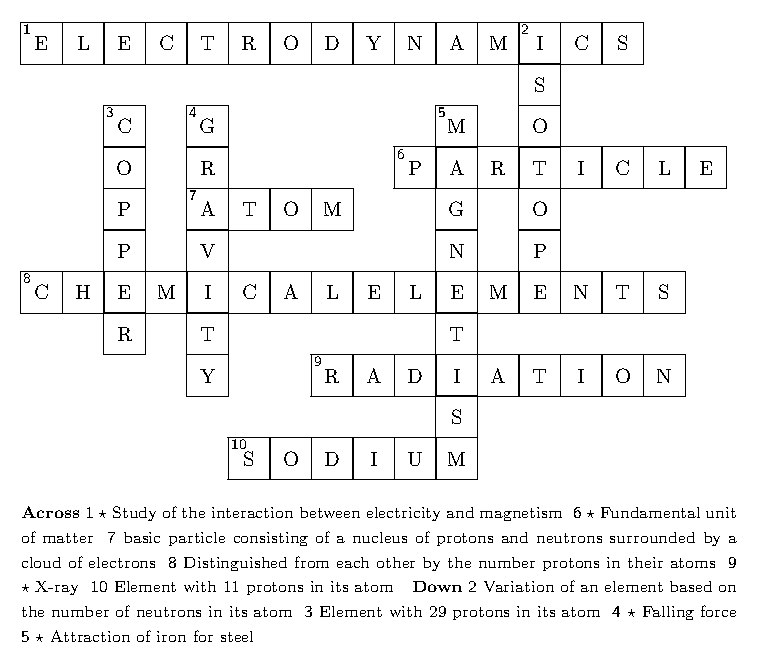
\includegraphics[width=0.85\textwidth]{figures/crossword.pdf}
  \end{columns}
\end{frame}

% --- 1.5 Our goal ---
\begin{frame}{Our Goal}
  \begin{center}
    \vspace{1em}
    \begin{tikzpicture}[
      box/.style={draw=unisired, rounded corners=8pt, minimum width=3.2cm, minimum height=1.5cm, align=center, font=\small\bfseries, text=unisired, line width=1pt},
      arr/.style={->, >=Stealth, line width=1.5pt, unisired!50}
    ]
    \node[box] (ai) at (0, 0) {Large Language\\Models};
    \node[box] (cross) at (5, 0) {Crossword\\Puzzles};
    \node[box] (edu) at (10, 0) {Educational\\Impact};
    \draw[arr] (ai) -- node[above, font=\scriptsize, text=graytext]{generate} (cross);
    \draw[arr] (cross) -- node[above, font=\scriptsize, text=graytext]{enhance} (edu);
    \end{tikzpicture}
    \vspace{2em}

    {\large An \textbf{end-to-end system} that automatically creates\\[0.3em]
    educational crosswords from text or keywords}
  \end{center}
\end{frame}